\cotefile{33}
\scanpage{98}
\unsure{supposons} $F$ \uline{constant}, puis (\unsure{le résolvant} par des $A_Y^n$) $F=A_Y$, mais alors le th est trivial.

b) Cas $f$ une immersion. Alors le th. est essentiellement trivial, sans hyp. de finitude.
En effet, on est ramené au cas d'une imm fermée. Alors
\[
\begin{aligned}
\mathbb R^{\unsure{!}}f^!(\mathbb R\mathcal Hom(F_\bullet,G^\bullet))
&\simeq f^!\deleted{\unsure{\mathbb R}}\underbrace{\mathcal Hom^\bullet(F_\bullet,C^\bullet(G^\bullet))}_{\substack{\text{N.B. c'est flasque,}\\\text{donc }f^!\text{-acyclique}}}\\
&\simeq \mathcal Hom^\bullet(f^*F_\bullet,\underbrace{f^!C^\bullet(G^\bullet)}_{\text{N.B. c'est injectif}})
\simeq\mathbb R\mathcal Hom(\mathbb Lf^*(F_\bullet),\mathbb R f^!(G^\bullet)).
\end{aligned}
\]

\figure{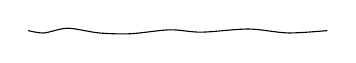
\begin{tikzpicture}[x=1cm,y=1cm]\draw plot[smooth] coordinates {(0,0)(.2,-.03)(.5,.03)(.9,-.03)(1.3,-.04)(1.8,.01)(2.2,-.02)(2.8,.02)(3.3,-.03)(3.8,0)};\end{tikzpicture}}

Les formules de projection \unsure{et bidualisation} comme \uline{formules de} \deleted{\unsure{commutation}\ \unsure{resp.}} \uline{d'échange}
\[
\left\{\begin{aligned}
\mathbb Rf_*D_X&\simeq D_Y\mathbb R_!f\\
\mathbb R^!fD_Y&\simeq D_X\mathbb Lf^*
\end{aligned}\right.
\]
i.e. $D$ ``échange'' $\mathbb Rf_*$ et $\mathbb R_!f$, $\deleted{\unsure{\mathbb R}}\mathbb Lf^*$ et $\mathbb L^!f$.

\mspage{97}
